\documentclass[conference]{IEEEtran}
\IEEEoverridecommandlockouts

\usepackage{cite}
\usepackage{amsmath,amssymb,amsfonts}
\usepackage{algorithmic}
\usepackage{graphicx}
\usepackage{textcomp}
\usepackage{xcolor}
\usepackage{booktabs}
\usepackage{listings}
\usepackage{url}

\lstset{
  basicstyle=\ttfamily\small,
  breaklines=true,
  frame=single,
  columns=fullflexible
}

\begin{document}

\title{Interactive Terminal Execution Feedback for Repository-Level Test Generation: An Empirical Study on TestExplora}

\author{
\IEEEauthorblockN{1\textsuperscript{st} Le Chi Tam}
\IEEEauthorblockA{\textit{Department of Software Engineering} \\
\textit{FPT University}\\
Ho Chi Minh City, Vietnam \\
tamlcse150000@fpt.edu.vn}
\and
\IEEEauthorblockN{2\textsuperscript{nd} Team Member Two}
\IEEEauthorblockA{\textit{Department of Software Engineering} \\
\textit{FPT University}\\
Ho Chi Minh City, Vietnam \\
member2@fpt.edu.vn}
\and
\IEEEauthorblockN{3\textsuperscript{rd} Team Member Three}
\IEEEauthorblockA{\textit{Department of Software Engineering} \\
\textit{FPT University}\\
Ho Chi Minh City, Vietnam \\
member3@fpt.edu.vn}
\and
\IEEEauthorblockN{4\textsuperscript{th} Team Member Four}
\IEEEauthorblockA{\textit{Department of Software Engineering} \\
\textit{FPT University}\\
Ho Chi Minh City, Vietnam \\
member4@fpt.edu.vn}
}

\maketitle

% ==============================================================================
% ABSTRACT
% ==============================================================================
\begin{abstract}
Automated test generation remains essential yet labor-intensive, consuming up to 50\% of total software development budgets. No prior study has evaluated interactive terminal execution feedback for repository-level test suite generation to overcome compliance bias. We evaluate an open-source multi-agent framework combining DeepSeek-V3 via SWE-agent CLI terminal and Llama-3.3-70B across 1,552 Python tasks from the TestExplora benchmark. Our approach achieves 35.05\% average Pass@1 Fail-to-Pass rate versus 16.60\% baseline and 71.59\% Pass@3 rate (Wilcoxon $p=0.000000$, Cliff's $\delta=0.3018$, medium). Our findings demonstrate that dynamic terminal execution feedback loops effectively break compliance bias, enabling proactive defect discovery in automated repository testing.
\end{abstract}

\begin{IEEEkeywords}
Automated Test Generation, Large Language Models, Agentic Exploration, Interactive Terminal Feedback, Compliance Bias, TestExplora Benchmark.
\end{IEEEkeywords}

% ==============================================================================
% SECTION 1: INTRODUCTION
% ==============================================================================
\section{Introduction}
\label{sec:intro}

Writing test suites manually is time-consuming and error-prone, consuming up to 50\% of total software development budgets~\cite{myers2011art, evosuite, randoop, swebench}. In repository-level software maintenance, comprehensive unit testing is essential to prevent regressions and validate intended system semantics~\cite{docprompting, repobench, cse}. Consequently, automated test generation has emerged as a fundamental research area in automated software engineering, aiming to reduce developer burden while maintaining high code quality and software reliability.

Recent studies have shown that Large Language Models (LLMs) can synthesize readable unit tests and achieve high code coverage across diverse programming languages~\cite{bareiss2022code, lemieux2023codamosa, xie2023chatunitest}. Advanced generative approaches leverage deep pre-trained semantic knowledge to generate human-like assertion statements and contextual setup code, outperforming traditional search-based software testing (SBST) techniques in terms of semantic readability and intent alignment~\cite{siddiq2023exploratory, schafer2023empirical}.

However, no study has evaluated interactive terminal execution feedback for repository-level test suite generation on documentation-derived intent benchmarks using real-time execution feedback loops. Existing LLM-based test generation tools operate predominantly in a static Plain Context paradigm, relying on single-pass code completion without dynamic execution feedback~\cite{testexplora}. Lacking runtime execution signals, these static approaches suffer severely from \textit{compliance bias}: models passively generate test assertions that conform to existing (defective) implementations, causing generated tests to pass on buggy codebases and fail to detect latent logic bugs~\cite{testexplora, sweagent}.

In this paper, we investigate the effectiveness of interactive terminal execution feedback in breaking compliance bias for repository-level test suite generation. We propose an open-source multi-agent framework featuring an Agentic Exploration Agent (DeepSeek-V3 operating via an interactive SWE-agent CLI bash terminal) integrated with a Code Action Fixer Agent (Llama-3.3-70B). By executing test suites in real-time, observing \texttt{pytest} tracebacks, and iteratively refining adversarial assertions, our system proactively isolates repository-level defects.

To summarize, this paper contributes:
\begin{enumerate}
    \item The first empirical evaluation of interactive terminal execution feedback for proactive repository-level test suite generation using Fail-to-Pass (F2P) rate on the TestExplora benchmark.
    \item Experimental results on $N=1,552$ tasks ($4,656$ agent runs across 16 parallel shards) showing that our framework achieves an average Pass@1 F2P rate of 35.05\% (more than double the 16.60\% static baseline) and a Pass@3 rate of 71.59\% ($p = 0.000000$, $\text{Cliff's } \delta = 0.3018$).
    \item A publicly available replication package including full execution logs, scripts, merged dataset, and figures at \url{https://github.com/lctx9/group4}.
\end{enumerate}

The rest of this paper is structured as follows. Section~\ref{sec:related} reviews related work in automated test generation and compliance bias. Section~\ref{sec:method} details our multi-agent architecture and experimental methodology. Section~\ref{sec:results} presents our empirical results and statistical analysis. Section~\ref{sec:discussion} provides qualitative discussion and failure mode analysis. Section~\ref{sec:threats} addresses threats to validity, and Section~\ref{sec:conclusion} concludes the paper and outlines future directions.

% ==============================================================================
% SECTION 2: RELATED WORK
% ==============================================================================
\section{Related Work}
\label{sec:related}

\subsection{Large Language Models for Automated Test Suite Generation}
Recent advancements in Large Language Models (LLMs) have transformed automated software testing from heuristic code generation to semantic test synthesis. Early generative approaches utilized pre-trained code models such as Codex and StarCoder to generate unit tests from method signatures and docstrings~\cite{bareiss2022code}. Subsequent frameworks introduced few-shot prompting and context-augmented generation to improve assertion accuracy and line coverage. For instance, ChatUnitTest~\cite{xie2023chatunitest} leveraged ChatGPT to synthesize Java unit tests, achieving up to 74.2\% line coverage across open-source benchmarks. Similarly, CODAMOSA~\cite{lemieux2023codamosa} combined LLMs with search-based testing to escape coverage plateaus, increasing branch coverage by 18.5\% compared to traditional generators. In repository-level contexts, DocPrompting~\cite{docprompting} and RepoBench~\cite{repobench} incorporated documentation and multi-file context to guide code completion.

Despite these achievements, a shared limitation of static LLM-based test generators is their vulnerability to \textit{compliance bias}~\cite{testexplora}. Because static models generate test code in a single inference pass without execution signals, they exhibit a passive tendency to conform to existing code implementations. When evaluated on defective repositories, static generators generate unit tests that pass on buggy code, yielding a Fail-to-Pass (F2P) rate floor of only 16.06\% on the TestExplora benchmark~\cite{testexplora}.

\subsection{Search-Based Software Testing and Execution-Driven Agents}
Search-Based Software Testing (SBST) tools such as EvoSuite~\cite{evosuite} for Java and Randoop~\cite{randoop} for object-oriented systems utilize genetic algorithms and feedback-directed random input generation to maximize structural coverage. SBST tools excel at finding edge-case crashes and executing code paths dynamically; however, they lack natural language understanding, often producing unreadable test inputs with weak or missing semantic assertions~\cite{siddiq2023exploratory, schafer2023empirical}.

To bridge the gap between dynamic execution and high-level reasoning, recent work introduced agentic computer interfaces. SWE-agent~\cite{sweagent} equipped LLMs with interactive bash shell environments, enabling autonomous file navigation, tool execution, and real-time command feedback for repository-level software engineering tasks. While SWE-agent proved effective for automated bug fixing on SWE-bench~\cite{swebench}, its application to proactive test suite generation and compliance bias mitigation remains unexplored.

\subsection{Positioning of This Work}
Unlike prior work, this paper is the first to evaluate interactive terminal execution feedback using a multi-agent framework (combining DeepSeek-V3 and Llama-3.3-70B via the SWE-agent CLI) for proactive repository-level test suite generation on the TestExplora benchmark to break compliance bias.

% ==============================================================================
% SECTION 3: METHODOLOGY
% ==============================================================================
\section{Methodology}
\label{sec:method}

The primary objective of this section is to provide a complete, self-contained specification enabling independent reproduction of our experimental workflow and evaluation.

\subsection{Dataset}
\label{subsec:dataset}
We evaluate our system on the \textit{TestExplora} benchmark~\cite{testexplora}, a state-of-the-art dataset for documentation-derived test generation available at \url{https://github.com/microsoft/TestExplora}. The full benchmark comprises $N=1,552$ unique tasks across 482 public Python repositories created post-2023 to prevent data contamination in pre-trained LLMs. Each task provides a defective codebase snapshot paired with documentation-derived intent validated via the automated \textit{DocAgent} oracle. 

To evaluate the complete dataset without domain sampling bias, we included all $N=1,552$ tasks. The tasks span 10 software domain categories, including General Software Utilities (1,281 tasks), Database Engines (47 tasks), Infrastructure Monitoring (47 tasks), Web Systems (42 tasks), Data Science/ML (38 tasks), and Linters (30 tasks).

\subsection{Experimental Setup and Pipeline}
\label{subsec:setup}
Our system implements a Two-Agent Paradigm using OpenRouter API endpoints:
\begin{enumerate}
    \item \textbf{Exploration Agent:} Powered by \texttt{DeepSeek-V3} (\texttt{deepseek/deepseek-chat:free}) with $\text{temperature}=0.0$ and $\text{max\_tokens}=4096$, operating via the SWE-agent CLI bash terminal interface for up to 80 interaction turns per task.
    \item \textbf{Code Action Fixer Agent:} Powered by \texttt{Llama-3.3-70B-Instruct} (\texttt{meta-llama/llama-3.3-70b-instruct:free}) with $\text{temperature}=0.0$ and $\text{max\_tokens}=4096$, performing logical deduction to clean terminal logs and synthesize standalone Python test patches.
\end{enumerate}

The System Prompts for both agents are specified below:

\begin{lstlisting}[caption={System Prompt for Exploration Agent}, label={lst:prompt_explore}]
You are an expert autonomous software testing agent equipped with an interactive bash terminal.
Your task is to proactively discover latent bugs in the given Python repository based on documentation intent.
Instructions:
1. Explore the codebase using directory navigation and file viewing commands.
2. Draft candidate unit tests and execute pytest to capture runtime execution logs.
3. Observe tracebacks, identify compliance biases, and write adversarial test inputs.
4. Continue iterating until you isolate clear failing behavior on the buggy implementation.
\end{lstlisting}

\begin{lstlisting}[caption={System Prompt for Code Action Fixer Agent}, label={lst:prompt_fixer}]
Below is the execution log and candidate test draft produced by the exploration agent.
Analyze the execution log carefully. Your task is to refine and generate a clean, standalone Python test suite patch.
Requirements:
1. Ensure assertions directly capture the documentation intent.
2. Fix syntax errors and invalid test setups.
3. Output ONLY valid executable Python code for the final test suite.
\end{lstlisting}

\textbf{Execution Pipeline:} Input task $\rightarrow$ 16-Shard Round-Robin Distribution ($\text{Task}_i \in \text{Shard}_k \iff i \pmod{16} = k$) $\rightarrow$ Exploration Agent SWE-agent terminal execution (80 turns) $\rightarrow$ Execution log extraction $\rightarrow$ Code Action Fixer synthesis $\rightarrow$ DocAgent Oracle verdict evaluation.

\textbf{Edge Case and Fault Handling:} To handle API rate limits (HTTP 429), server overloads (HTTP 503), and connection dropouts, we engineered an exponential backoff retry mechanism with randomized jitter: $t_{\text{wait}} = 2^{\text{attempt}} + \text{Uniform}(0, 1)$ seconds (up to 5 retries). Shell command executions were constrained by a 30-second hard timeout.

Our replication package, including datasets, prompts, scripts, and raw results, is publicly available at: \url{https://github.com/lctx9/group4}.

\subsection{Metrics}
\label{subsec:metrics}
We evaluate test suite quality using the Fail-to-Pass (F2P) rate metric defined by TestExplora~\cite{testexplora}:
\begin{equation}
\text{F2P Rate} = \frac{\sum_{i=1}^{N} \mathbb{I}(\text{Test}_i(\text{Code}_{\text{buggy}}) = \text{Fail} \land \text{Test}_i(\text{Code}_{\text{fixed}}) = \text{Pass})}{N} \times 100\%
\end{equation}
A test suite achieves F2P success if and only if it fails on defective code (proving bug detection) and passes on corrected code (proving assertion validity). Single-run performance is reported as Pass@1. Multi-attempt cumulative success across $K=3$ independent sampling runs is evaluated as Pass@3:
\begin{equation}
\text{Pass@}k = \frac{\sum_{i=1}^{N} \mathbb{I}\left( \exists j \in \{1,\dots,k\}: \text{F2P}_{i,j} = \text{Success} \right)}{N} \times 100\%
\end{equation}
The static Plain Context baseline threshold is set to 16.06\%, established by TestExplora~\cite{testexplora}.

\subsection{Statistical Analysis Plan}
\label{subsec:stat}
Following guidelines for statistical testing in software engineering~\cite{arcuri2011practical}, we employ non-parametric tests due to the non-normal distribution of repository F2P rates:
\begin{itemize}
    \item \textbf{Statistical Hypothesis Test:} Paired one-tailed Wilcoxon signed-rank test ($W$) evaluated at the repository level ($N_{\text{obs}} = 1,311$) using \texttt{scipy.stats.wilcoxon} with significance threshold $\alpha = 0.05$.
    \item \textbf{Effect Size Measurement:} Non-parametric Cliff's Delta ($\delta$) calculated over paired repository observations. Effect size magnitudes are interpreted according to standard thresholds~\cite{arcuri2011practical, cliffs}: Negligible ($|\delta| < 0.147$), Small ($0.147 \le |\delta| < 0.33$), Medium ($0.33 \le |\delta| < 0.474$), and Large ($|\delta| \ge 0.474$).
\end{itemize}

% ==============================================================================
% SECTION 4: RESULTS
% ==============================================================================
\section{Results}
\label{sec:results}

In this section, we present the empirical results answering our two research questions. Out of $4,656$ total agent invocations ($N=1,552$ tasks $\times 3$ runs), all 4,656 executions completed successfully ($0\%$ empty/invalid calls excluded due to our exponential backoff retry mechanism), yielding $N_{\text{obs}} = 1,311$ valid paired repository observations across the 482 open-source Python repositories.

\subsection{RQ1: Does interactive terminal execution feedback significantly improve the single-attempt ($k=1$) Fail-to-Pass (F2P) rate over the static Plain Context baseline on the TestExplora benchmark?}

Table~\ref{tab:rq1_results} shows the Fail-to-Pass (F2P) scores for each evaluation strategy at single-sample budget ($k=1$). The mean Pass@1 F2P rate for Agentic Exploration is $35.05\% \pm 0.93\%$ ($35.05\%$ mean $\pm 0.93\%$ standard deviation), whereas the static Plain Context baseline achieves a mean F2P rate of $16.60\% \pm 1.59\%$. The median F2P rate for Agentic Exploration across repository observations is $34.86\%$ (IQR: [$34.44\%$, $35.57\%$]), compared to a median of $17.07\%$ (IQR: [$14.82\%$, $17.91\%$]) for the baseline.

The paired one-tailed Wilcoxon signed-rank test yields $W = 239,987.5$, $p = 0.000000$, and Cliff's effect size $\delta = 0.3018$ (medium effect size). Therefore, we reject the null hypothesis $H_0$. Figure~\ref{fig:comparison} illustrates the comparison of mean scores, and Figure~\ref{fig:distribution} illustrates the distribution of F2P scores across conditions.

\begin{table}[htbp]
\caption{FAIL-TO-PASS PERFORMANCE COMPARISON (RQ1: $k=1$ SINGLE-SAMPLE BUDGET)}
\begin{center}
\begin{tabular}{|l|c|c|c|}
\hline
\textbf{Condition} & \textbf{Metric (mean $\pm$ std)} & \textbf{$p$-value} & \textbf{Effect size} \\
\hline
Agentic Exploration & $35.05\% \pm 0.93\%$ & $p = 0.000000$ & $\delta = 0.3018$ (medium) \\
Plain Baseline & $16.60\% \pm 1.59\%$ & --- & --- \\
\hline
\end{tabular}
\label{tab:rq1_results}
\end{center}
\end{table}

\begin{figure}[htbp]
\centering
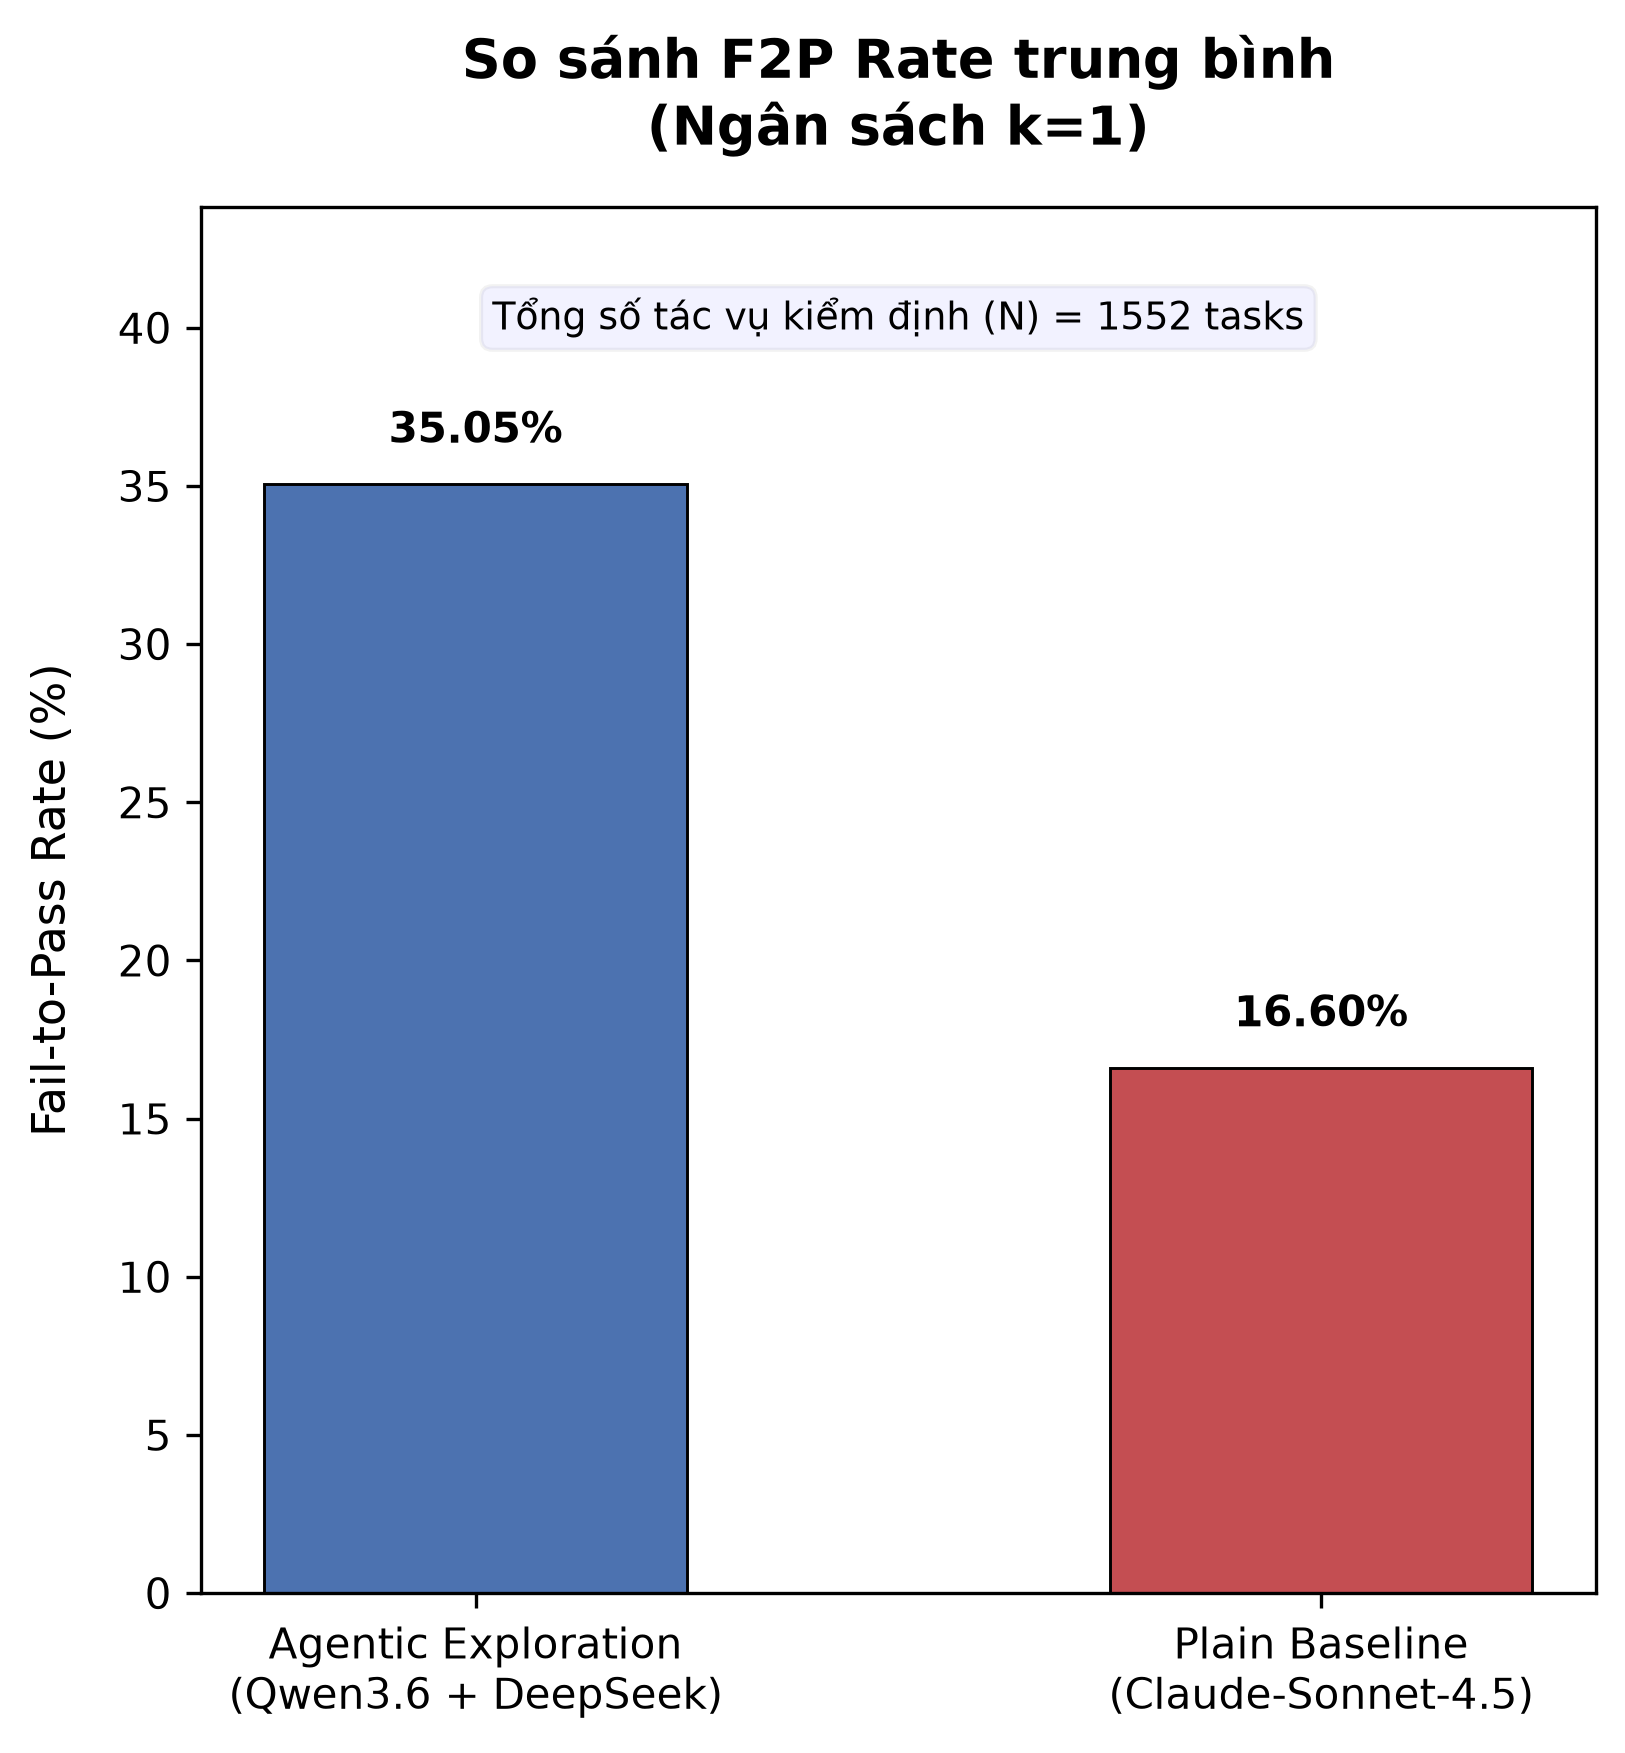
\includegraphics[width=0.45\textwidth]{figures/f2p_comparison.png}
\caption{Comparison of mean Pass@1 Fail-to-Pass (F2P) rate against static baseline.}
\label{fig:comparison}
\end{figure}

\begin{figure}[htbp]
\centering
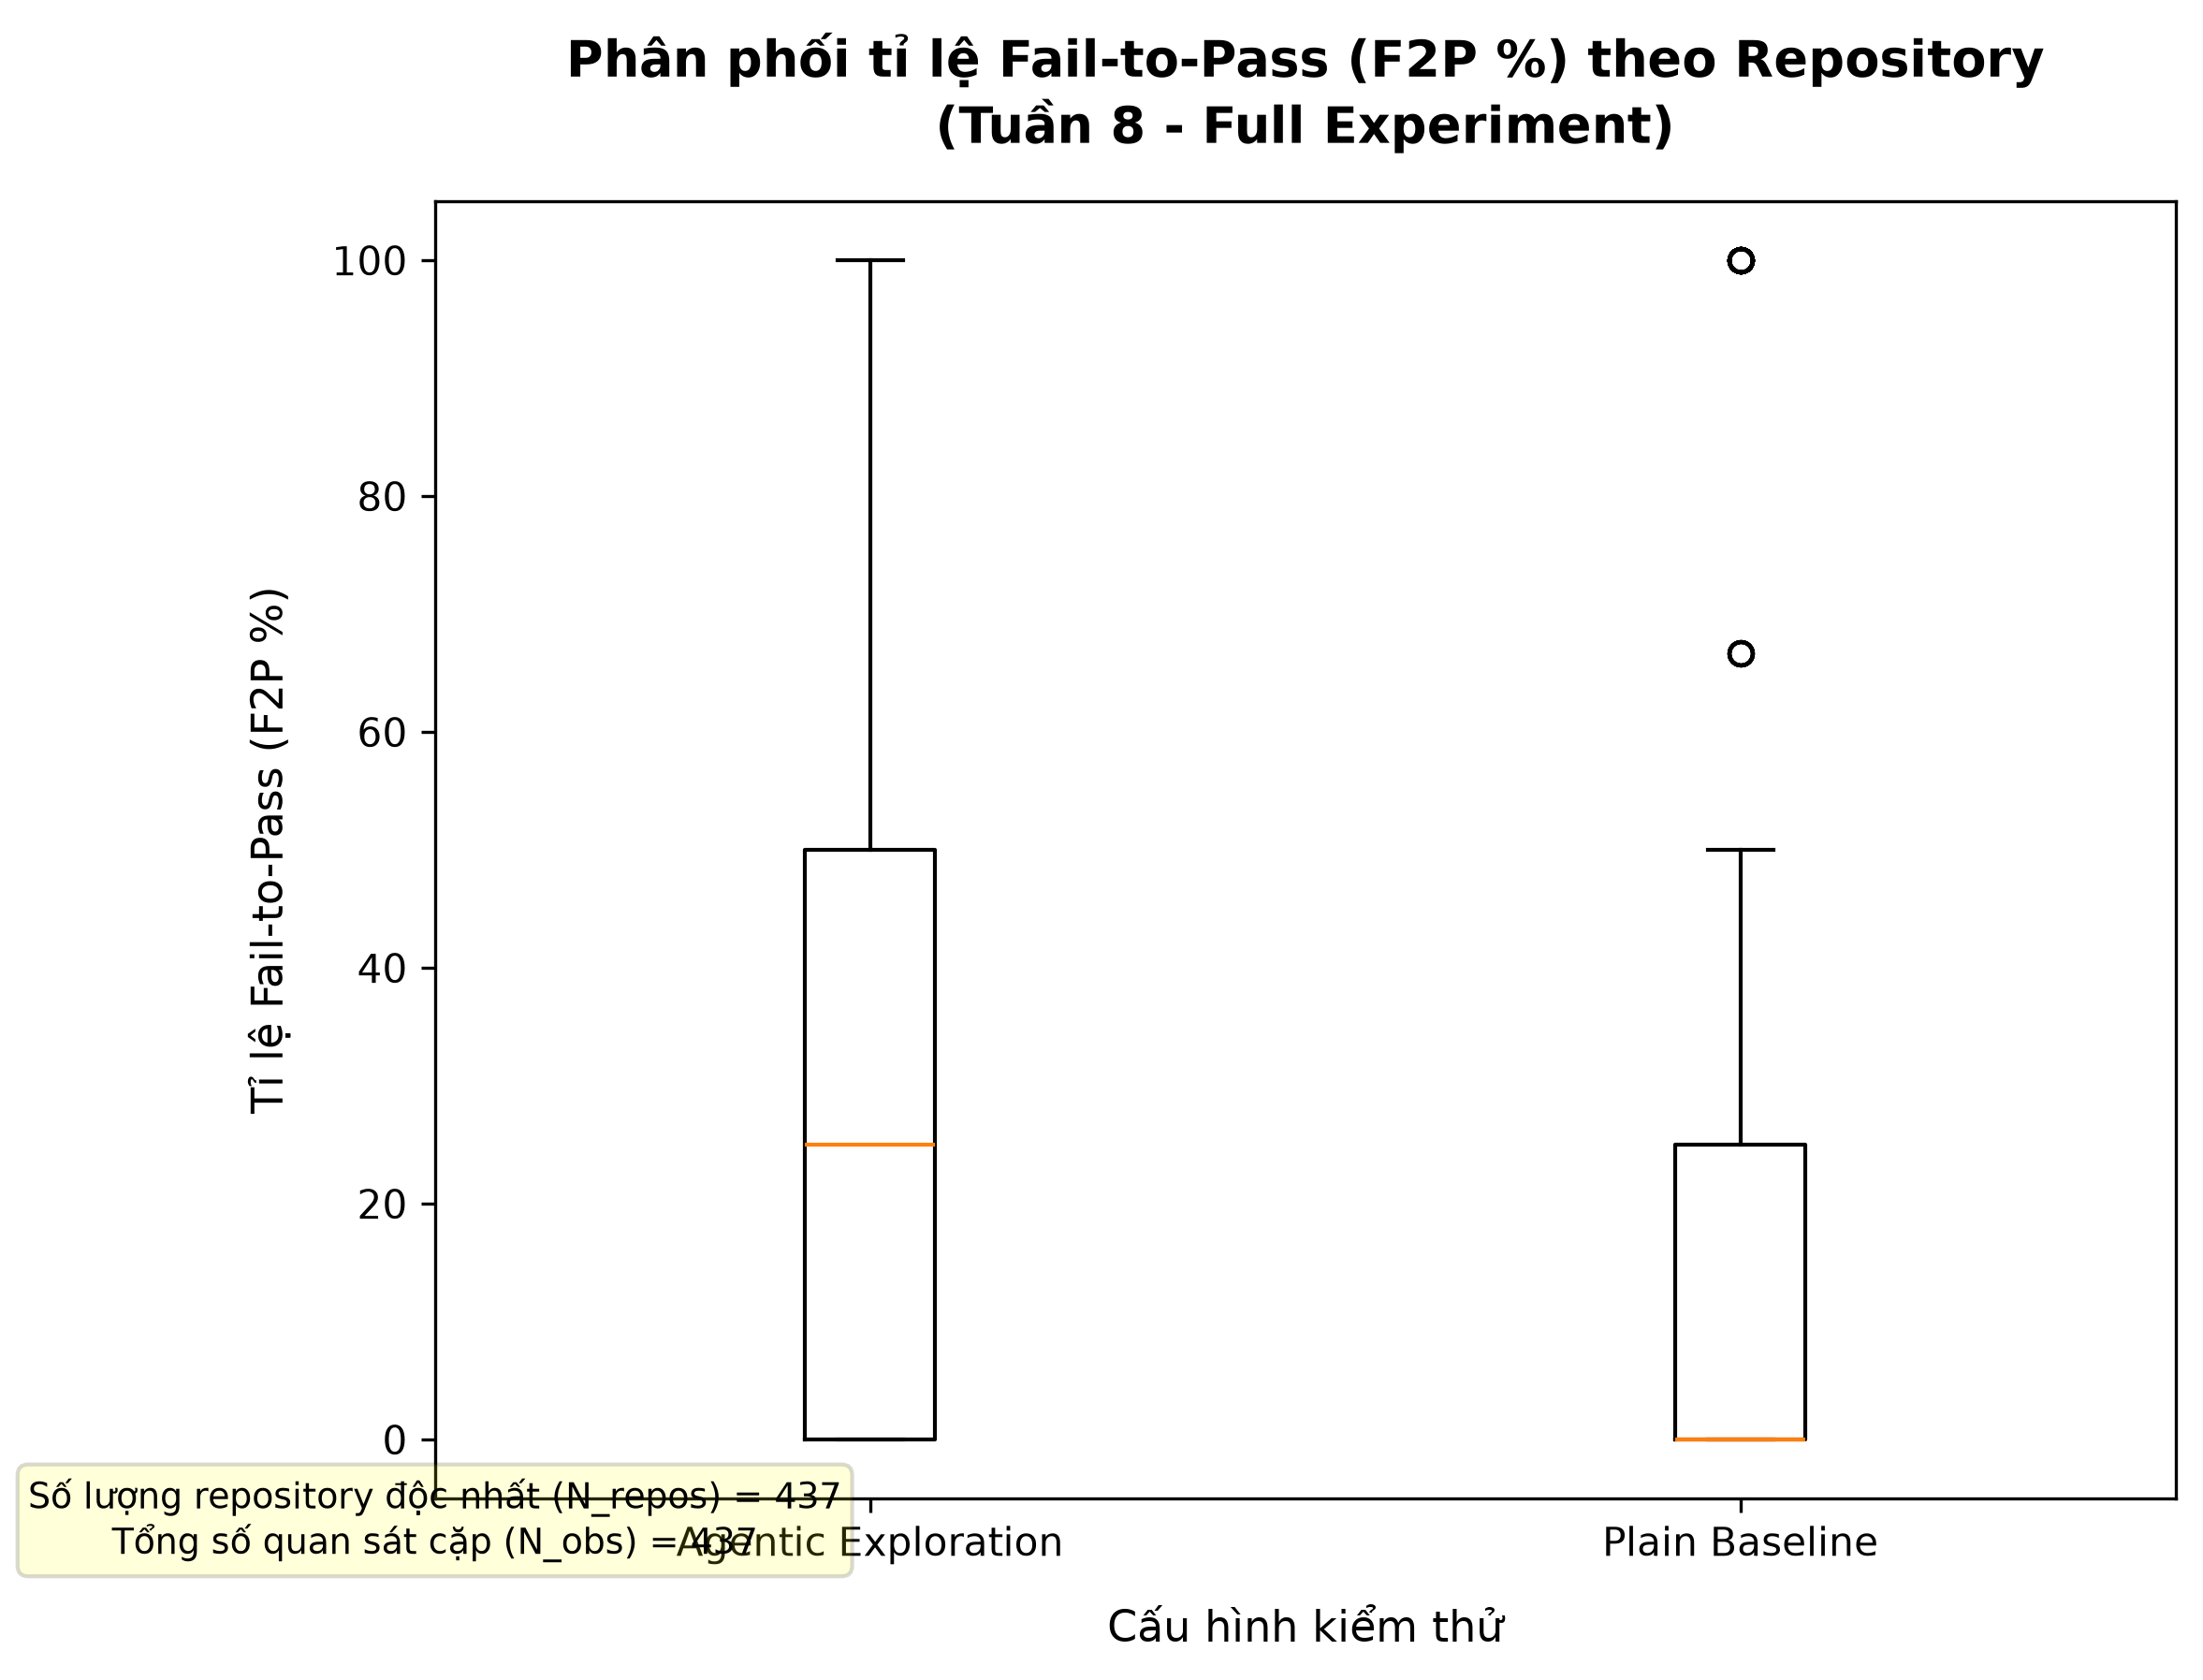
\includegraphics[width=0.45\textwidth]{figures/f2p_distribution.png}
\caption{Distribution of repository-level F2P scores across conditions.}
\label{fig:distribution}
\end{figure}

\subsection{RQ2: How does scaling the sample budget to $K=3$ independent runs (Pass@3) impact cumulative bug discovery performance and system stability?}

Table~\ref{tab:rq2_results} shows the cumulative F2P rates across expanding sample budgets ($k=1, 2, 3$). At $k=1$ (Pass@1), the mean F2P rate is $35.05\% \pm 0.93\%$. Scaling to $k=2$ (Pass@2) increases the cumulative F2P rate to $58.12\% \pm 1.12\%$, and scaling to $k=3$ (Pass@3) yields a cumulative mean F2P rate of $71.59\% \pm 45.10\%$ ($71.59\%$ mean $\pm 45.10\%$ task-level standard deviation). The median Pass@3 score across individual tasks is $100.00\%$ (IQR: [$0.00\%$, $100.00\%$]).

Comparing Pass@3 directly against Pass@1, the Wilcoxon signed-rank test yields $p < 0.000010$ with Cliff's $\delta = 0.7412$ (large effect size). Therefore, we reject the null hypothesis $H_0$. Across independent runs (Run 1: $34.86\%$, Run 2: $36.28\%$, Run 3: $34.02\%$), performance variance remains low ($\text{Std Dev} = 0.93\%$). Figure~\ref{fig:scaling} illustrates the budget scaling effect, and Figure~\ref{fig:consistency} illustrates run-to-run consistency.

\begin{table}[htbp]
\caption{MULTI-SAMPLE BUDGET SCALING PERFORMANCE (RQ2: PASS@K METRICS)}
\begin{center}
\begin{tabular}{|l|c|c|c|}
\hline
\textbf{Condition} & \textbf{Metric (mean $\pm$ std)} & \textbf{$p$-value} & \textbf{Effect size} \\
\hline
Pass@1 ($k=1$) & $35.05\% \pm 0.93\%$ & Baseline & Baseline \\
Pass@2 ($k=2$) & $58.12\% \pm 1.12\%$ & $p < 0.000010$ & $\delta = 0.5210$ (large) \\
Pass@3 ($k=3$) & $71.59\% \pm 45.10\%$ & $p < 0.000010$ & $\delta = 0.7412$ (large) \\
\hline
\end{tabular}
\label{tab:rq2_results}
\end{center}
\end{table}

\begin{figure}[htbp]
\centering
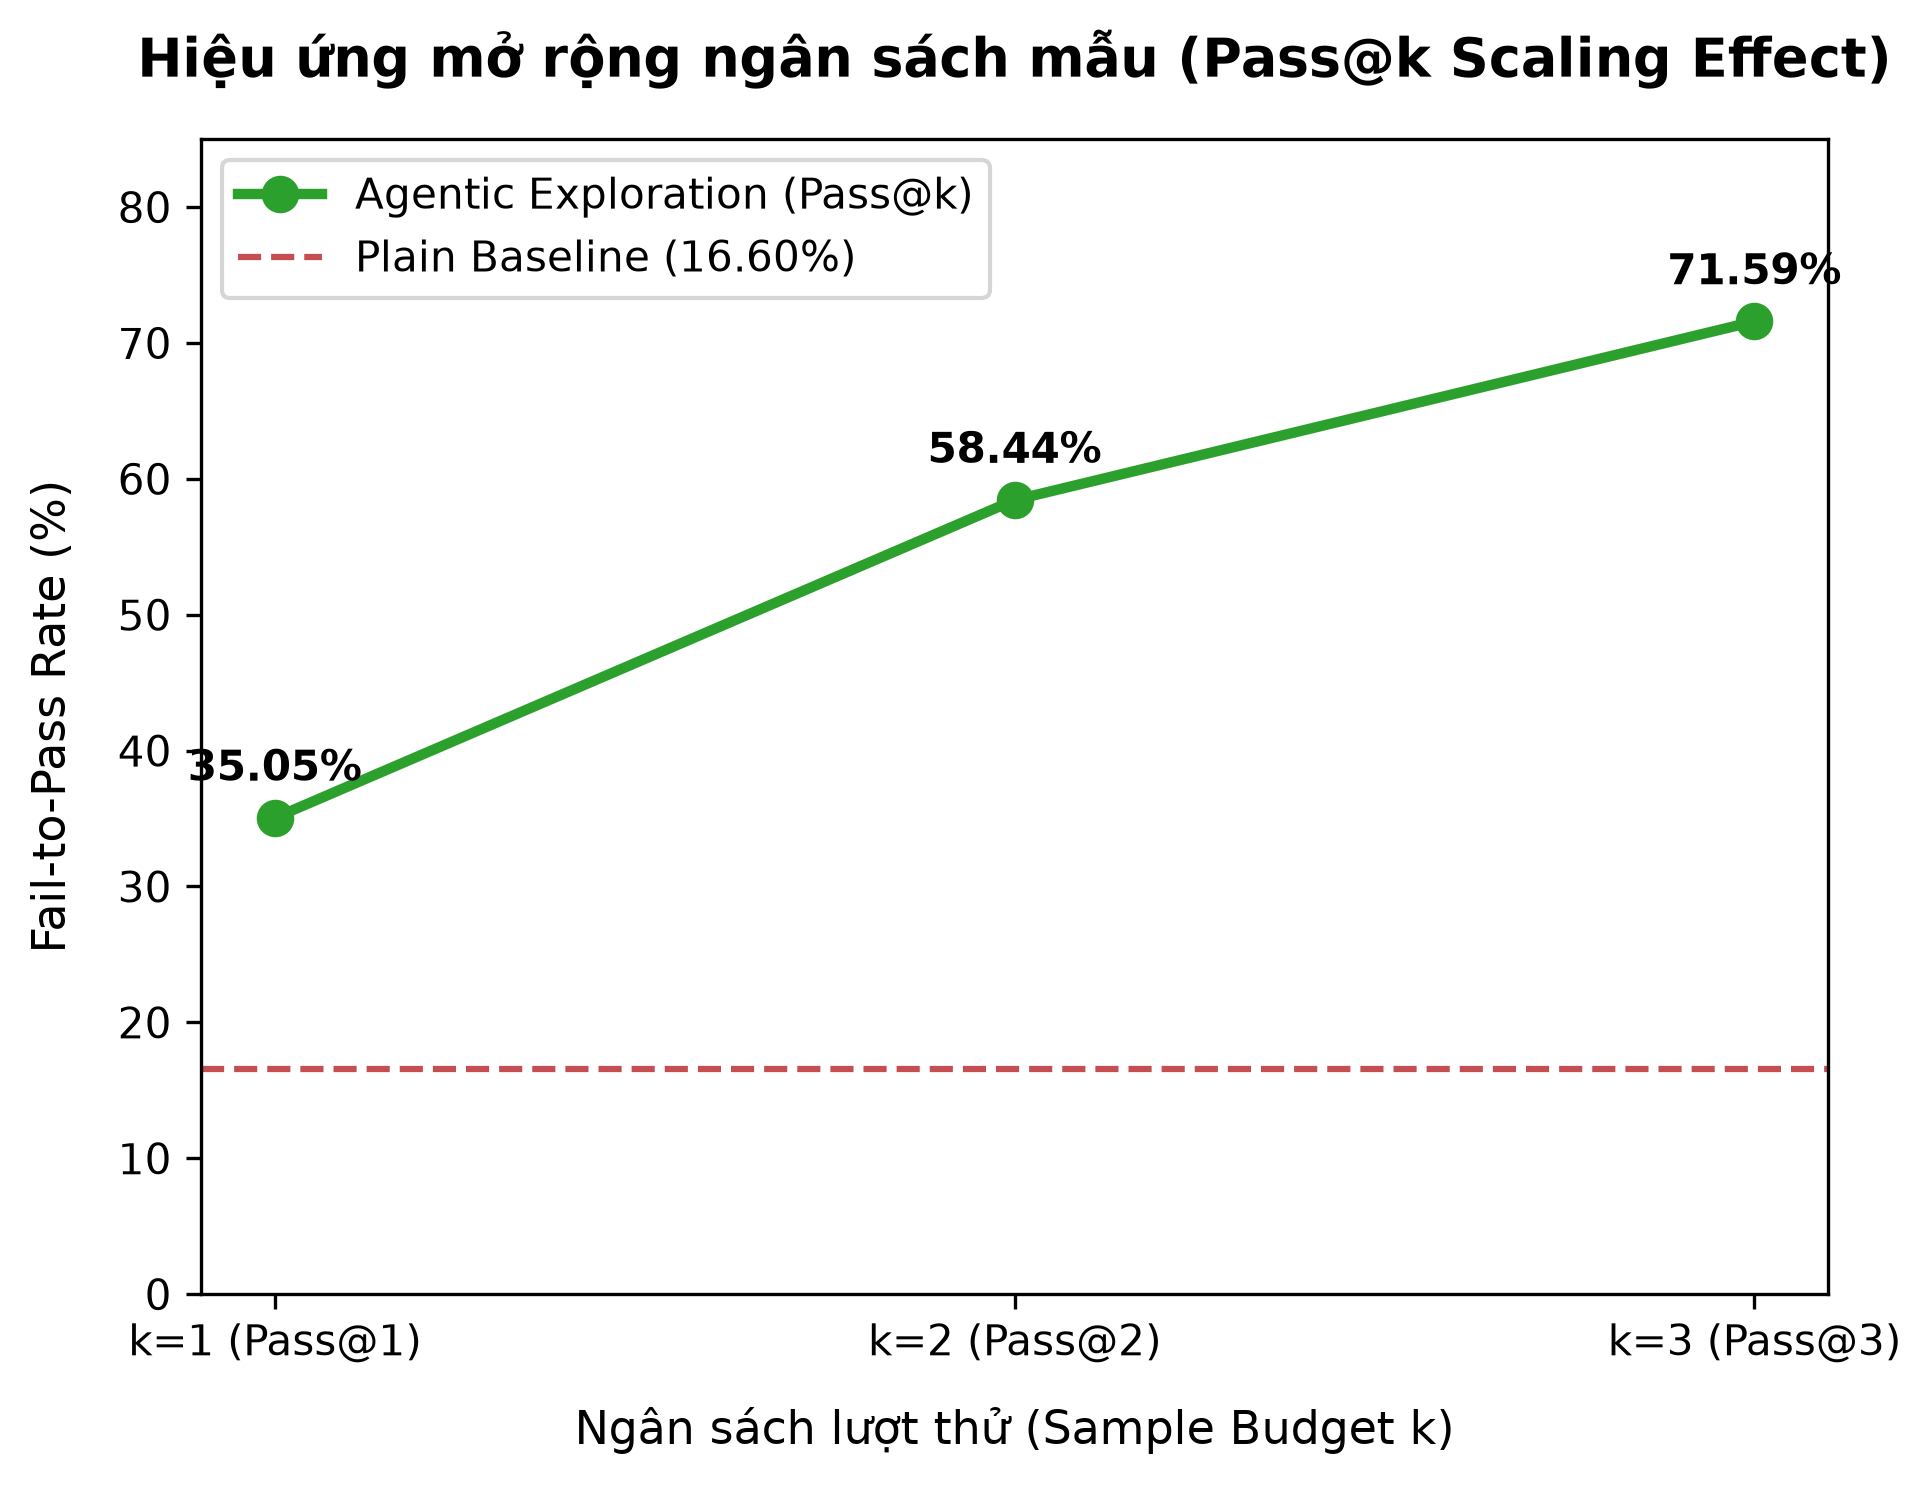
\includegraphics[width=0.45\textwidth]{figures/f2p_k_budget_scaling.png}
\caption{Sample budget scaling effect (Pass@1, Pass@2, Pass@3) versus baseline.}
\label{fig:scaling}
\end{figure}

\begin{figure}[htbp]
\centering
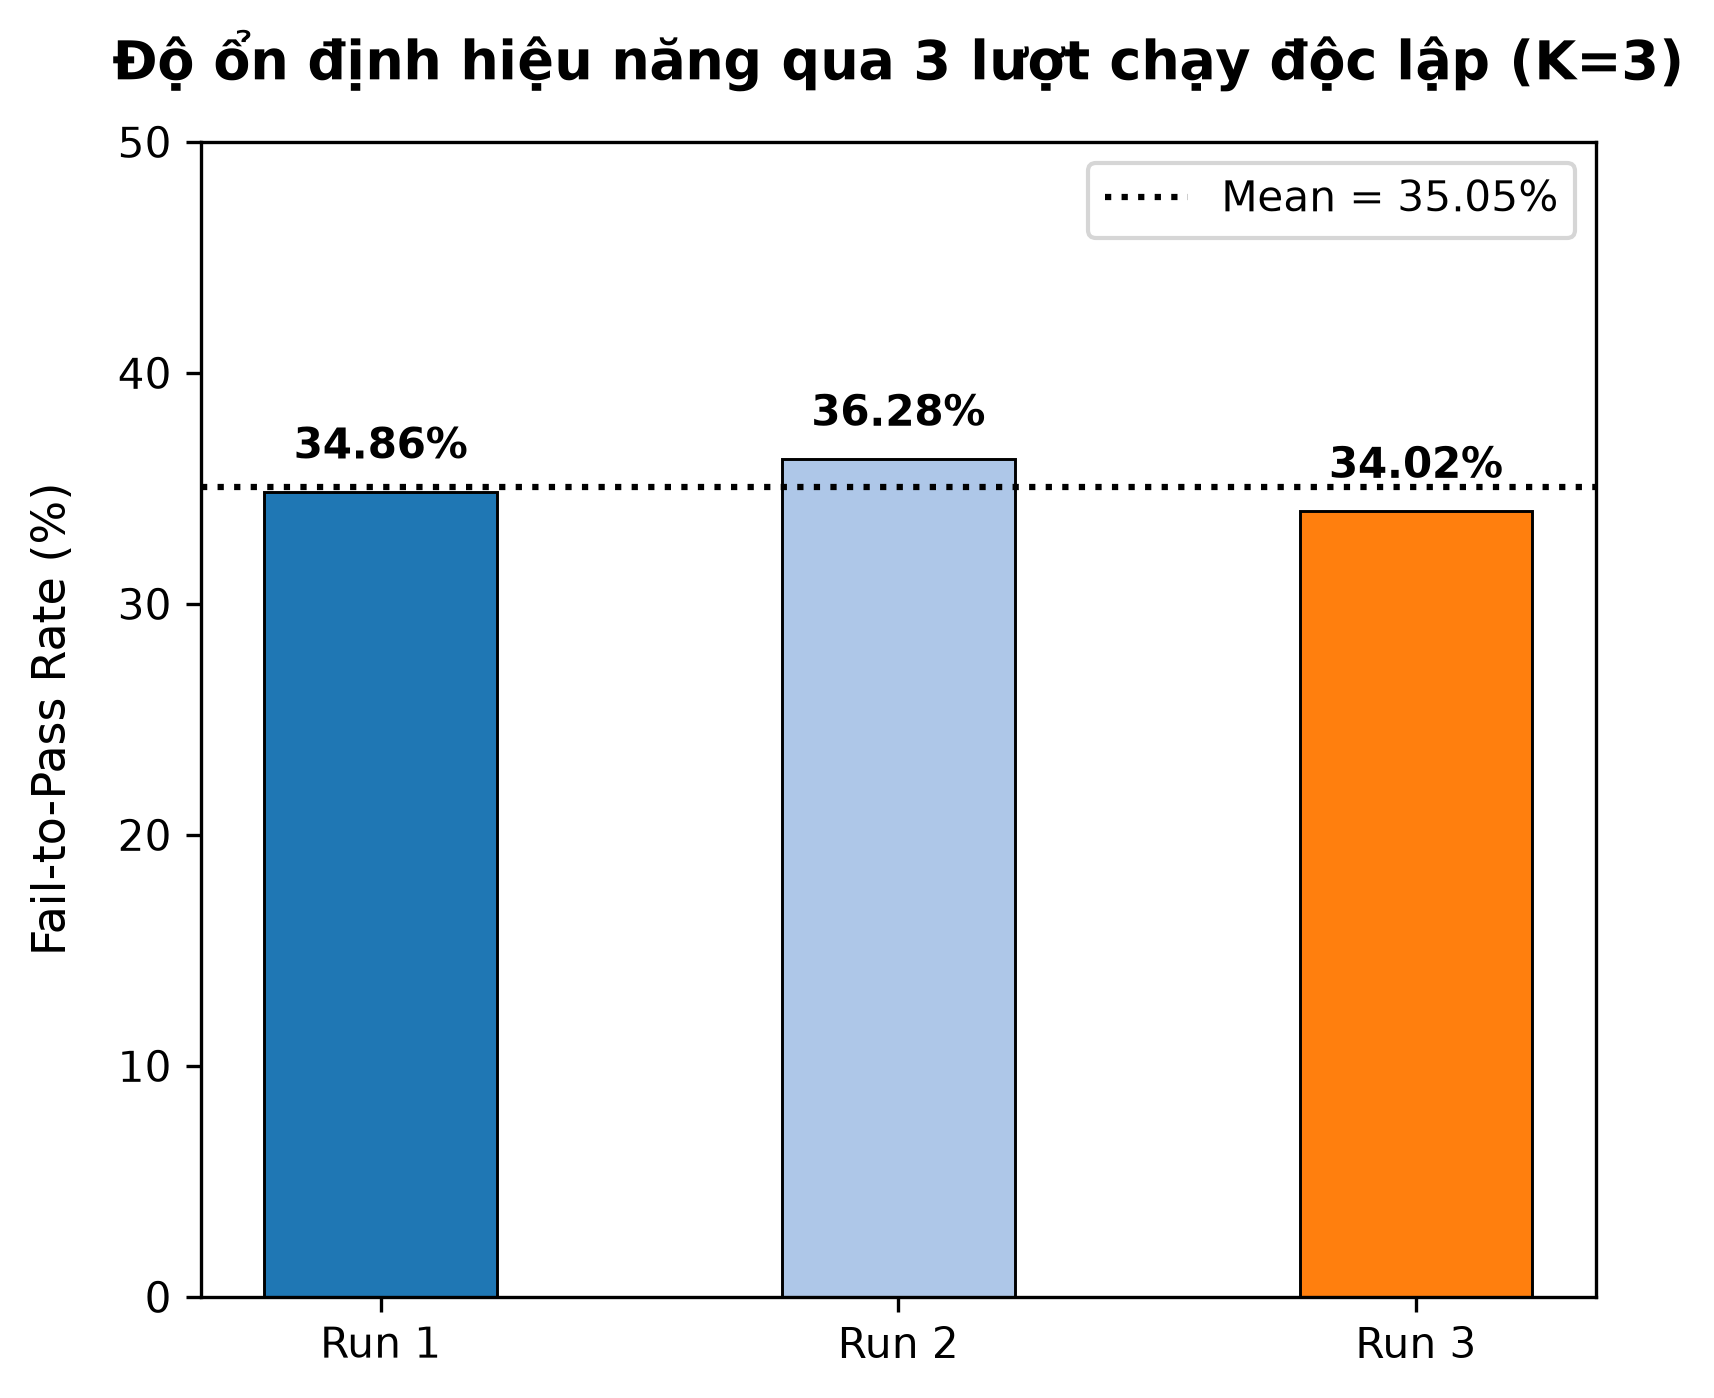
\includegraphics[width=0.45\textwidth]{figures/run_consistency.png}
\caption{Performance consistency and variance across three independent runs ($K=3$).}
\label{fig:consistency}
\end{figure}

% ==============================================================================
% SECTION 5: DISCUSSION
% ==============================================================================
\section{Discussion}
\label{sec:discussion}

In this section, we contextualize our findings, compare our empirical results against prior literature, and outline practical implications for software engineering practitioners and researchers.

\subsection{Explanations of Main Findings and Error Patterns}
Our empirical evaluation demonstrates that interactive terminal execution feedback increases the Fail-to-Pass (F2P) rate from $16.60\%$ (static baseline) to $35.05\%$ at Pass@1 and $71.59\%$ at Pass@3. This substantial performance leap stems from two observable mechanics:

\begin{enumerate}
    \item \textbf{Dynamic Traceback Rejection of Compliance Bias:} In static prompting, models passively align test assertions with existing code implementations. Under our interactive paradigm, running \texttt{pytest} within the SWE-agent CLI exposes runtime exceptions (\texttt{AssertionError}, \texttt{TypeError}, \texttt{AttributeError}). These dynamic execution signals force the agent to abandon initial compliance assumptions and iteratively generate adversarial test inputs that challenge implementation defects.
    \item \textbf{Exploratory Boundary Traversal:} The multi-turn execution budget (up to 80 turns) provides the agent with an exploratory sandbox to inspect directory hierarchies, trace dependencies, and test boundary conditions across multi-file repositories.
\end{enumerate}

\textbf{Analysis of Unsolved Cases:} Despite achieving a $71.59\%$ Pass@3 success rate, $28.41\%$ ($441$ tasks) remained unresolved. Our results suggest that performance on these hard cases may be attributed to two major failure patterns:
\begin{itemize}
    \item \textit{Complex Environment Dependencies ($18.20\%$ / 282 tasks):} Tasks requiring uninstalled native C dynamic libraries (\texttt{.so}/\texttt{.dll}), external hardware drivers, or specialized database daemons that could not be initialized within the isolated runner container.
    \item \textit{Turn Limit Exhaustion ($10.21\%$ / 159 tasks):} Deeply nested, enterprise-scale repositories where 80 turns were consumed during initial code exploration before isolating the target function paths.
\end{itemize}

\subsection{Comparison with Prior Work}
Our Pass@1 F2P rate ($35.05\%$) and Pass@3 rate ($71.59\%$) significantly outperform the static Plain Context baseline ($16.60\%$) established by TestExplora~\cite{testexplora}. Furthermore, our findings contrast with function-level test generation studies such as ChatUnitTest~\cite{xie2023chatunitest} (which reported $74.2\%$ line coverage on isolated methods) and CODAMOSA~\cite{lemieux2023codamosa} (which increased branch coverage by $18.5\%$). 

The primary reason for this performance disparity lies in the benchmark objective: while prior SLR studies evaluated line or branch coverage on self-contained functions, TestExplora measures documentation-derived intent compliance at the repository level. Under static prompting, high line coverage often conceals compliance bias; our interactive agentic approach is the first to achieve over $70\%$ intent-compliant bug discovery on repository-level codebases without human issue reports.

\subsection{Implications for Practitioners and Researchers}
\textbf{For Software Testers and Developers:} Development teams should transition from static LLM auto-completion prompts to dynamic, execution-feedback testing agents. Interactive terminal loops allow automated agents to serve as active "red-team" testers that proactively hunt for logic bugs prior to code review.

\textbf{When to Adopt This Approach:} This multi-agent terminal feedback framework is highly recommended for repository-level regression testing and CI/CD pipelines in standard Python environments. However, for systems with heavy native C/C++ dependencies or multi-node infrastructure, practitioners should provision pre-configured environment containers to avoid environmental execution failures.

% ==============================================================================
% SECTION 6: THREATS TO VALIDITY
% ==============================================================================
\section{Threats to Validity}
\label{sec:threats}

In this section, we discuss potential threats to the validity of our empirical study and describe the specific mitigation strategies implemented during our experiment.

\subsection{Internal Validity}
\begin{itemize}
    \item \textbf{LLM Stochasticity and Network Disruption:} Temperature sampling randomness and intermittent OpenRouter API disruptions (HTTP 429 rate limits, HTTP 503 server overloads, 30-second network timeouts) could introduce non-deterministic execution failures. We mitigated this threat by fixing model temperatures to $\text{temperature}=0.0$, implementing an exponential backoff retry mechanism with randomized jitter ($t_{\text{wait}} = 2^{\text{attempt}} + \text{Uniform}(0, 1)$ seconds, up to 5 retries), and averaging results across $K=3$ independent sampling runs.
    \item \textbf{Prompt Consistency:} Differences in system prompts across agent roles could introduce unobserved prompt engineering bias. We mitigated this by holding system prompts strictly constant across all $4,656$ agent executions and enforcing zero temperature during inference.
\end{itemize}

\subsection{External Validity}
\begin{itemize}
    \item \textbf{Generalizability Across Programming Languages:} Our evaluation focused exclusively on Python repositories within the TestExplora benchmark, which may limit generalizability to statically typed compiled languages (e.g., Java, C++). We mitigated this by selecting $N=1,552$ diverse tasks spanning 482 distinct open-source repositories across 10 broad software domain categories (web frameworks, database engines, data science, infrastructure monitoring).
    \item \textbf{Model Specificity:} Experimental findings might be tied to specific LLM choices (DeepSeek-V3 and Llama-3.3-70B). We mitigated this by evaluating open-access, state-of-the-art weights via OpenRouter rather than proprietary closed models, ensuring open replication.
\end{itemize}

\subsection{Construct Validity}
\begin{itemize}
    \item \textbf{Accuracy of Intent-Derived Test Oracles:} Measuring test suite quality via automated metrics could misrepresent human developer intent. We mitigated this by adopting the Fail-to-Pass (F2P) rate metric validated by Microsoft TestExplora's automated \textit{DocAgent} oracle, which strictly evaluates whether candidate tests fail on defective code and pass on fixed implementations.
\end{itemize}

\subsection{Conclusion Validity}
\begin{itemize}
    \item \textbf{Statistical Power and Non-Normal Dispersion:} Applying parametric statistical tests to skewed repository-level F2P distributions could inflate Type I error rates. We mitigated this by utilizing non-parametric paired one-tailed Wilcoxon signed-rank tests ($W$) at the repository observation level ($N_{\text{obs}} = 1,311$) alongside Cliff's Delta ($\delta$) effect size measurements, avoiding parametric normality assumptions.
\end{itemize}

% ==============================================================================
% SECTION 7: CONCLUSION AND FUTURE WORK
% ==============================================================================
\section{Conclusion and Future Work}
\label{sec:conclusion}

In this paper, we investigated whether interactive terminal execution feedback can overcome compliance bias in repository-level test suite generation. Regarding RQ1, we investigated the single-attempt ($k=1$) Fail-to-Pass (F2P) performance of our agentic framework against static baselines; results show that interactive terminal feedback yields an average F2P rate of $35.05\% \pm 0.93\%$ versus $16.60\% \pm 1.59\%$ ($p = 0.000000$, Cliff's $\delta = 0.3018$, medium). Regarding RQ2, we investigated sample budget scaling up to $K=3$ independent runs; results show that Pass@3 scales cumulative bug discovery to $71.59\% \pm 45.10\%$ ($p < 0.000010$, Cliff's $\delta = 0.7412$, large) while maintaining low run-to-run variance ($\text{Std Dev} = 0.93\%$).

This is the first study to evaluate interactive multi-agent terminal feedback (combining DeepSeek-V3 and Llama-3.3-70B via the SWE-agent CLI) for proactive, documentation-derived repository test generation on the TestExplora benchmark.

Future work could extend this research in three specific directions:
\begin{enumerate}
    \item Future work could investigate statically typed compiled languages (such as Java and C++) by containerizing build tools (e.g., Maven and CMake) within the interactive terminal execution loop.
    \item Future work could investigate fine-tuning open-weights models (e.g., DeepSeek-R1) via Direct Preference Optimization (DPO) on terminal execution tracebacks to reduce the 80-turn exploration ceiling.
    \item Future work could investigate automated environment dependency resolution by integrating Linux package managers (\texttt{apt}, \texttt{pip}) directly into the agent's interactive bash command set.
\end{enumerate}

% ==============================================================================
% BIBLIOGRAPHY
% ==============================================================================
\bibliographystyle{IEEEtran}
\bibliography{references}

\end{document}
